\documentclass{article}
\usepackage[utf8]{inputenc}

\title{SHiP Shield Review}
\author{fedor.ratnikov }
\date{April 2019}

\usepackage{natbib}
\usepackage{graphicx}

\begin{document}

\maketitle

\section{Muon shield}

This muon shield is designed to reduce the flux of muons by six orders of magnitude 
in the detector acceptance. The shield consists of a first set of magnets that deflect the 
positively and negatively 
charged muons on either side of the beam axis, irrespective of their initial 
direction. This allows creating a region around the beam line beyond this first set of 
magnets in which there are no charged particles. A second set of magnets which have 
their return field in this unoccupied region then provides further deflection. This 
configuration prevents muons deflected in the first section from being deflected back 
towards the detector by the return field in the second section.  

Since the Technical Proposal (TP), the muon shield design has seen two major updates.
Firstly, the separation of positive and negative muons in the first section of the shield 
can be achieved in the shortest distance by the application of a magnetic field as 
soon as the muons are produced. While it is not practically possible to magnetise 
the target in the SHIP set-up, the new design includes a magnetisation of the hadron
stopper. Secondly, with this addition, the field configuration of the entire set of 
free-standing magnets has been re-optimised with the help of machine learning techniques.
The resulting system of magnets is now $35\,m$ long (compared to the TP design of 48\,m) 
and has 1400\,T of magnets (previously 2900\,T). 
The reduced length of the shield gives the detector a larger geometric acceptance for 
signal decays for a given transverse size of the spectrometer. 

\subsection{Free-standing muon shield}

The design of the muon shield and the residual rate of muons depends on the momentum 
distribution of the muons produced in the initial proton collision. The latest shield 
optimisation and rate estimates were performed using extensive full MC simulations with 
Pythia and GEANT, and Machine Learning techniques. In order to validate these 
simulations an experiment was performed in summer 2018 (Section~\ref{sec:muflux}) 
to measure the muon spectrum using a replica of SHiP's target~\cite{SHiP-EOI-016} 
(\ref{sec:muon_flux_measurement}). The optimisation was based on the use of Grain-Oriented (GO) steel allowing 
a high magnetic flux density at a very limited current (FIGURE). Grain-oriented steel 
sheets comes in $0.3 - 0.5\,mm$ thickness. Taking into account the packing factor 
and other imperfections it was estimated that an average field of $1.7\,T$ could be 
achieved throughout the magnets. By default, the machine learning started from a 
free-standing muon shield consisting of six magnets, each of $\sim 5\,$m length, separated 
by 10\,cm gaps. The geometry of each magnet is described by XXX parameters. In total there are therefore around 40 parameters that describe the geometry. 
The geometric parameters are optimised by minimising 
a loss function that reduces both the number of muons entering into the decay volume and the 
resulting weight. The simulation sample used for this optimisation is formed from $\sim$18M 
muons produced in the target which, for each iteration of the optimisation, are propagated 
through a full GEANT simulation of the detector. The optimisation is extremely CPU intensive 
and a Bayesian optimisation procedure is therefore employed rather than a conventional 
gradient approach~\cite{}. Despite the large simulation sample, the optimisation is 
statistically limited with only a handful of muons passing through the final shield 
configuration. The optimised shield design is shown in Figure~\ref{}. The trajectory of a 
muon that passes through the shield and forms the residual muon background is shown in Figure~\ref{}. A large-angle multiple scatter
in the first part of the shield causes this positive/negative muon to move to the ``wrong'' side
of the beam line and the second part of the shield then focuses it towards the detector.

\begin{figure}[tbh]
\centering
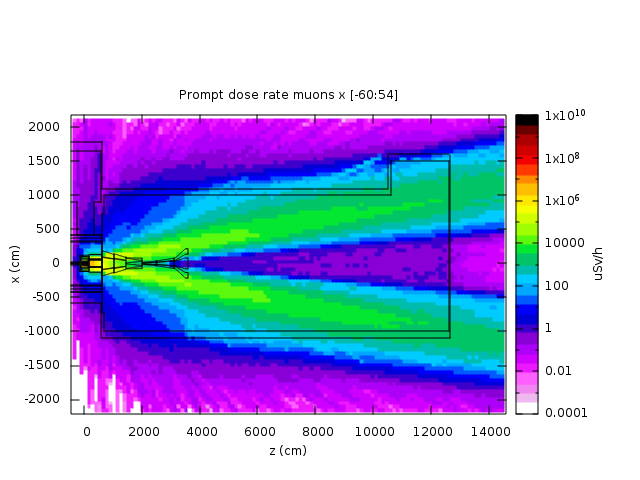
\includegraphics[width=0.7\columnwidth]{figs/2018_10_03_MuonFlux_FLUKA.png}
\caption{TO BE UPDATED WITH LATEST SIMULATION}
\label{fig:MuonShieldFluka}
\end{figure}

The re-optimised parameters of the magnets obtained from the machine learning has been
used to build a 3D CAD model of the muon shield (Figure~\ref{fig:3dView}) assuming the 
characteristics of grain-oriented steel. The model was used to produce a realistic magnetic 
field simulation with the OPERA~\cite{ref:OPERA_magnetic_simulation} package. 
Figure~\ref{fig:shieldMagneticField} shows the calculated magnetic field in a cross-section of
the muon shield. The  magnetic field simulation shows a good homogeneity and strength in 
the regions critical for deflecting the high momentum muons and minor degradation in the
less important outer regions. 

The very high permeability is very sensitive to high temperatures and high mechanical 
stresses. For these reasons the design and performance of the free-standing muon shield 
magnets with the help of GO steel pose a number of technological challenges. These 
include how to best assemble sheets of GO steel without disrupting the magnetic 
circuit, how to cut the GO sheets into desired configurations, and how to best connect the 
GO sheets to achieve the desired stacking factor. In order to address these questions a 
prototyping campaign is underway.

The tentative design of a magnet body entirely made from GO steel sheets is illustrated in 
Figure~\ref{fig:shieldConstruction}. It consists of 50 mm thick packs of sheets connected 
together by riverts, spot welding or alternatively screws. Packs are bolted together into 
rectangular blocks of about 50 cm depth. One block is thus made of about 1000 metal sheets
of the same size. This makes mass production of such sheets reasonable cheap. Finally, 
blocks of different shapes are installed on the support beams.  Figure~\ref{fig:fullMechanics}
shows a tentative design of the shield constructed as a set of rectangular blocks.
Welding by electron beam technology is tentatively chosen for connecting sections together.
Dedicated tests have been made to measure magnetic properties of actual GO steel samples, 
as well as possible degradation of these properties by the welding procedure. Green lines 
in Figure~\ref{fig:goSteelAnnealing} shows the measured properties of the initial GO steel in the direction of and perpendicular to the grain structure. The blue line corresponds to the sample that has been welded by the electron beam. The magnetic 
quality of the welded sample degrades significantly.
The microscopic image in Figure~\ref{fig:goCarbonStructure} shows the carbon structure which 
appeared in the joint after the welding. An annealing process to reduce the tension and to restore the material properties was tested.
Annealing at $500^\circ$C and at $700^\circ$C were separately applied to the welded test 
samples. It demonstrated that it was possible to recover most of the original magnetic 
properties of the material (Figure~\ref{fig:goSteelAnnealing}).

The continued R\&D and prototyping program aims at determining the degradation of the magnetic 
properties in the critical regions of the magnet in larger scale assemblies which includes
the structural elements. Another critical factor which requires careful consideration is the
stacking factor that may be achieved in the full assemblies. Figure~\ref{fig:shieldEffectiveField} 
shows the effective magnetic field in the critical volume of the first magnet of the shield 
by comparing the case with ideal jointing of the GO steel sheets with the case based on the 
measured magnetic properties of welded joints. Stacking factors of 95\% and 90\% have been
assumed. First calculations show minor degradation of the overall magnet performance 
despite the relatively significant degradation of the field in the joints. 
Figure~\ref{fig:shieldEffectiveField} shows the actual map of the magnetic fields in the different 
assumptions. The electrical current is chosen to provide an effective field of $1.7~,T$ in the 
critical region.

In complement to the studies of magnet yokes constructed entirely from GO steel, a hybrid solution
is also pursued with GO steel in the critical region of the magnet surrounded by a return yoke of
a normal iron with good magnetic properties.



% Anizotropic magnetic properties of the GO steel are important for the shield construction, as this allows to make 
% magnetic field of strength about 1.8 T in solid body, that cooresponds to about 1.7 T effective magnetic field considering
% unavoidable sheet packing factor. That strong field is necessary to deflect highest momentum muons that may be 
% produced in the target. Different sections across the magnet must have different grain orientation, thus corresponding pieces
% must be connected to form magnetically connected sections with different anizotropy orientation.
% It is well known however that strong mechanical or thermal impact can degrade or destroy the anizotropy structure
% of the GO steel. 

\begin{figure}[thbp]
\centering
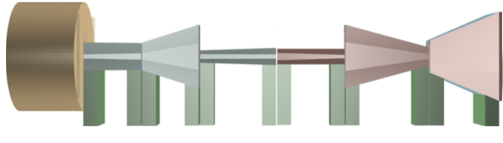
\includegraphics[width=0.9\columnwidth]{figs/shield_YZview.png}
\caption{Side view of the optimised muon shield magnets.}
\label{fig:shieldSideView}
\end{figure}

\begin{figure}[thbp]
\centering
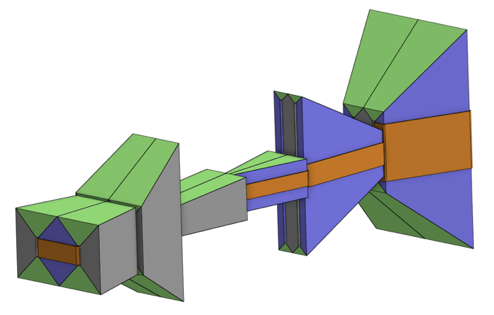
\includegraphics[width=0.7\columnwidth]{figs/shield_3dview.png}
\caption{3D view of the optimised muon magnetic shield. Description ????}
\label{fig:3dView}
\end{figure}

\begin{figure}[thbp]
\centering
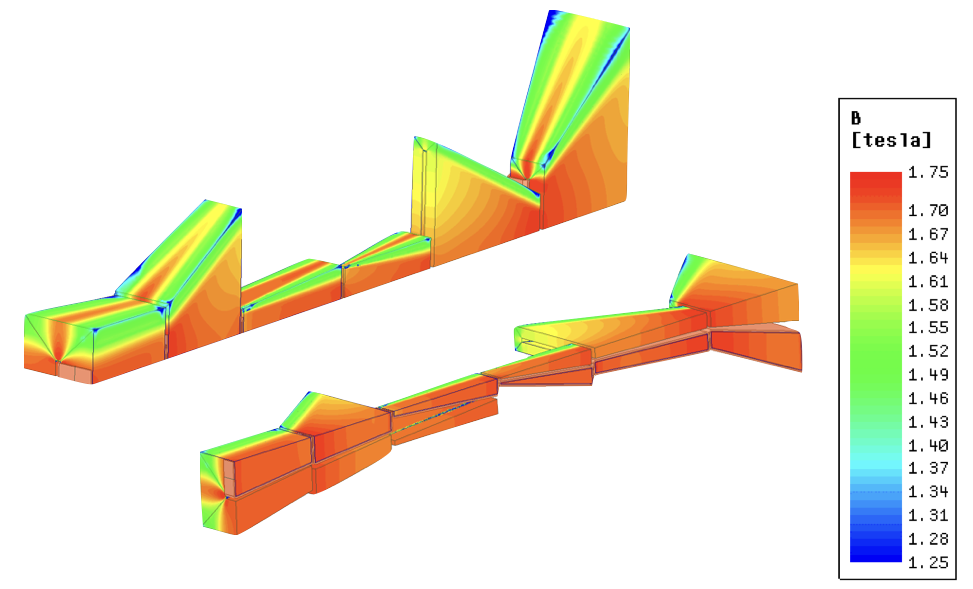
\includegraphics[width=0.8\columnwidth]{figs/shield_field_quadrant.png}
\caption{Modelled magnetic field distribution with nominal field intensity set to 1.7T. Quadrant cut out is shown.}
\label{fig:shieldMagneticField}
\end{figure}

\begin{figure}[thbp]
\centering
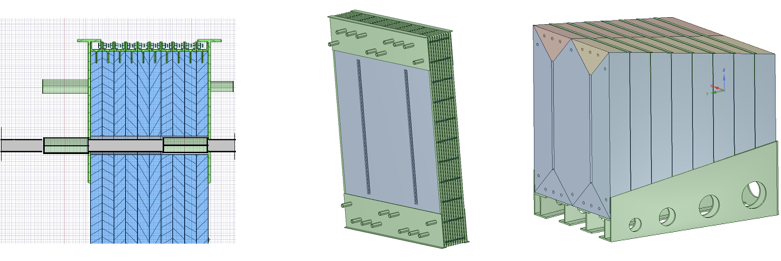
\includegraphics[width=0.8\columnwidth]{figs/shieldConstruction.png}
\caption{Tentative mechanical design of magnets. GO steel sheets are packed into sections about 50 mm thick (left). 
Packs are bolted together into rectangular block about 50 cm thick (left, central). blocks of different dimensions are installed on the support beams (right).}
\label{fig:shieldConstruction}
\end{figure}

\begin{figure}[thbp]
\centering
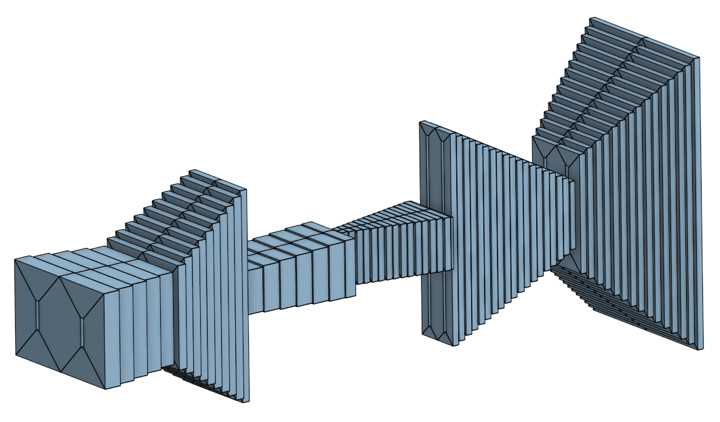
\includegraphics[width=0.7\columnwidth]{figs/fullMechanics.png}
\caption{Tentative construction of the muon shield made of rectangular blocksfullMechanics.png.}
\label{fig:fullMechanics}
\end{figure}

\begin{figure}[thbp]
\centering
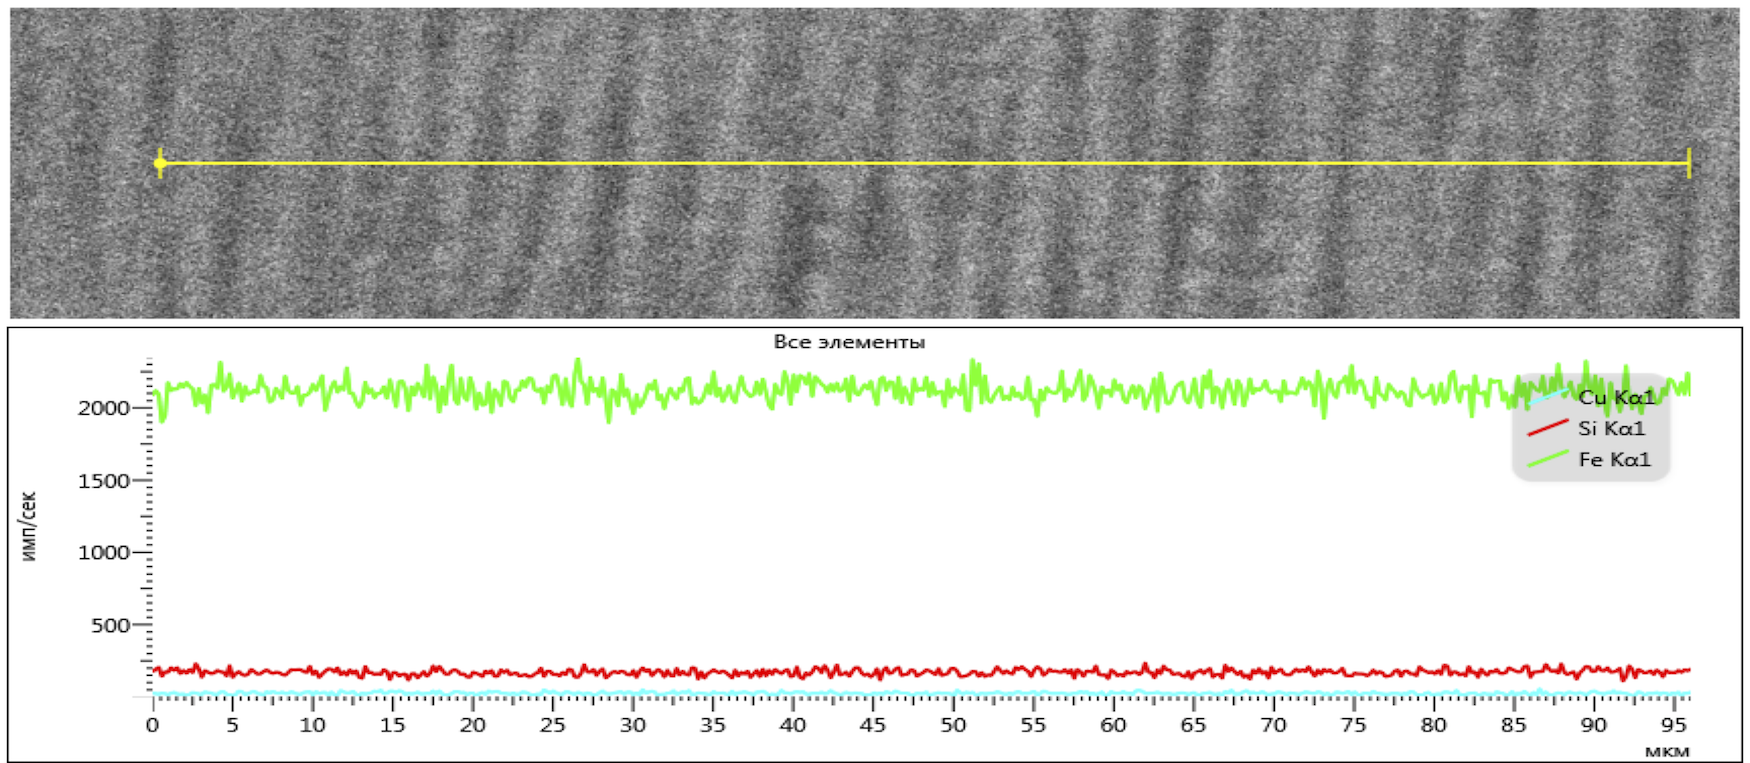
\includegraphics[width=0.7\columnwidth]{figs/carbon_structure.png}
\caption{Carbon structure in the welded joint before the annealing.}
\label{fig:goCarbonStructure}
\end{figure}

\begin{figure}[thbp]
\centering
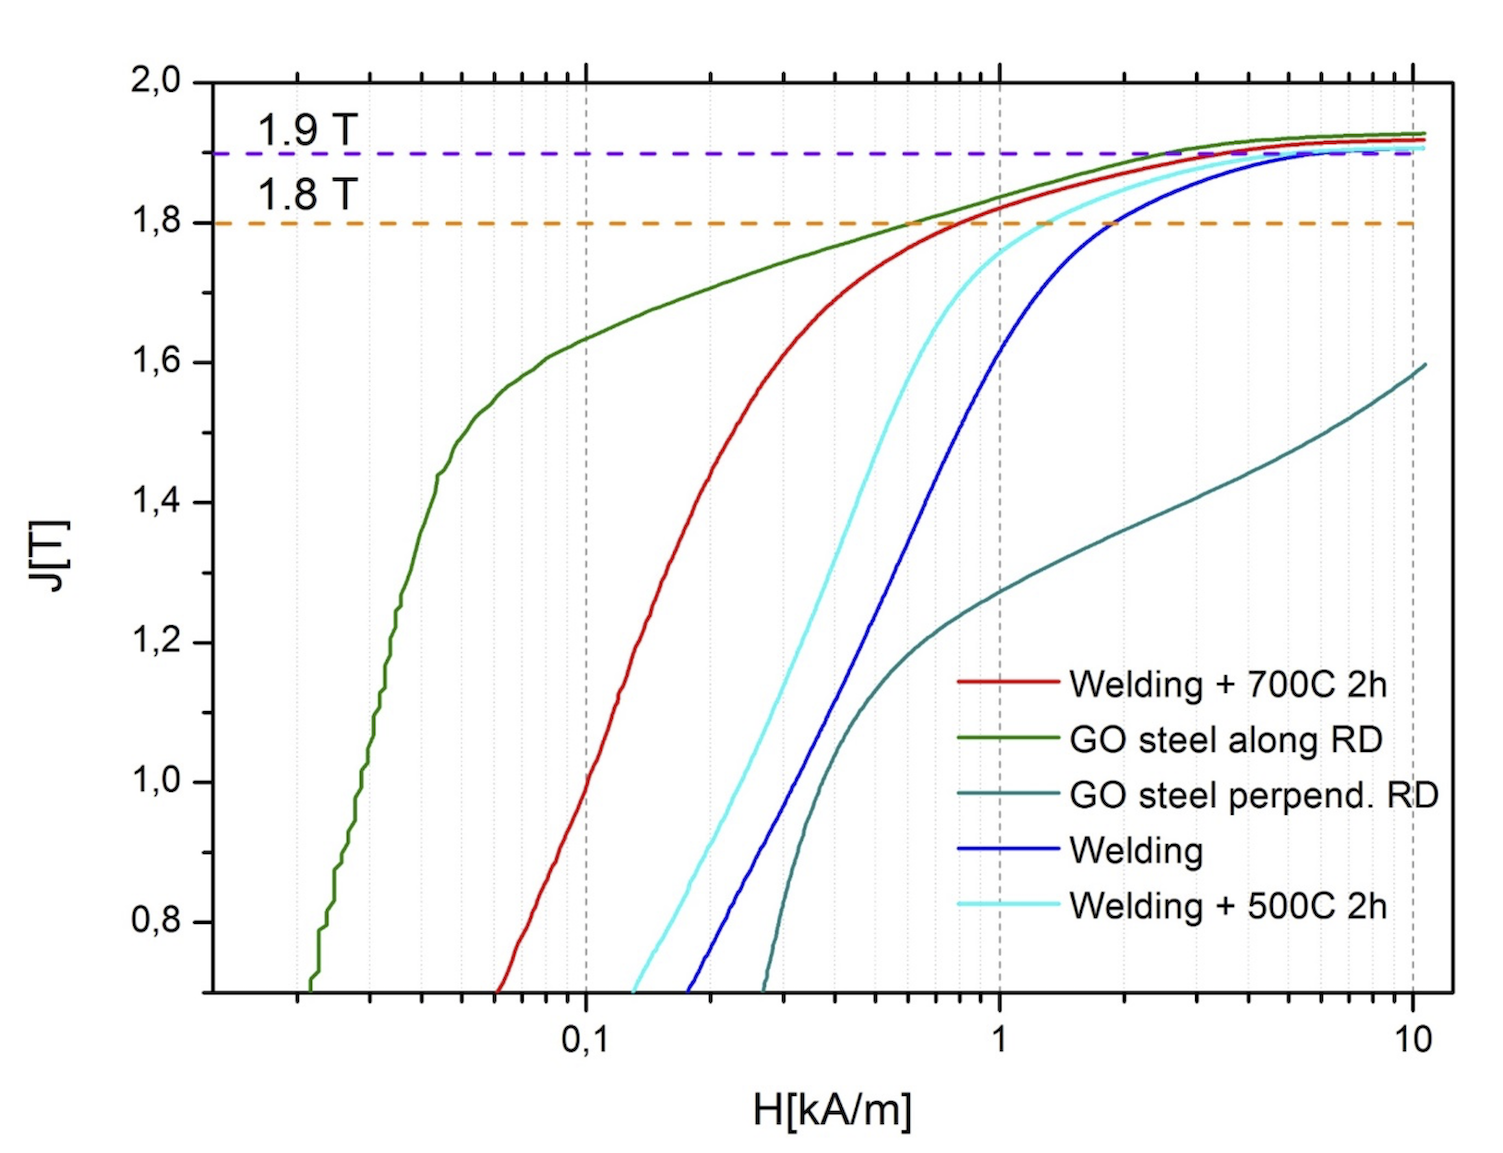
\includegraphics[width=0.6\columnwidth]{figs/go_steel_annealing.png}
\caption{Measured magnetic properties of the Grain Oriented steel batch: unprocessed sample along (green) and perpendicular (dark green) to rolling direction,
after the welding (blue), after the following annealing at $500^\circ$C (cyan) and $700^\circ$C (red).}
\label{fig:goSteelAnnealing}
\end{figure}


\begin{figure}[thbp]
\centering
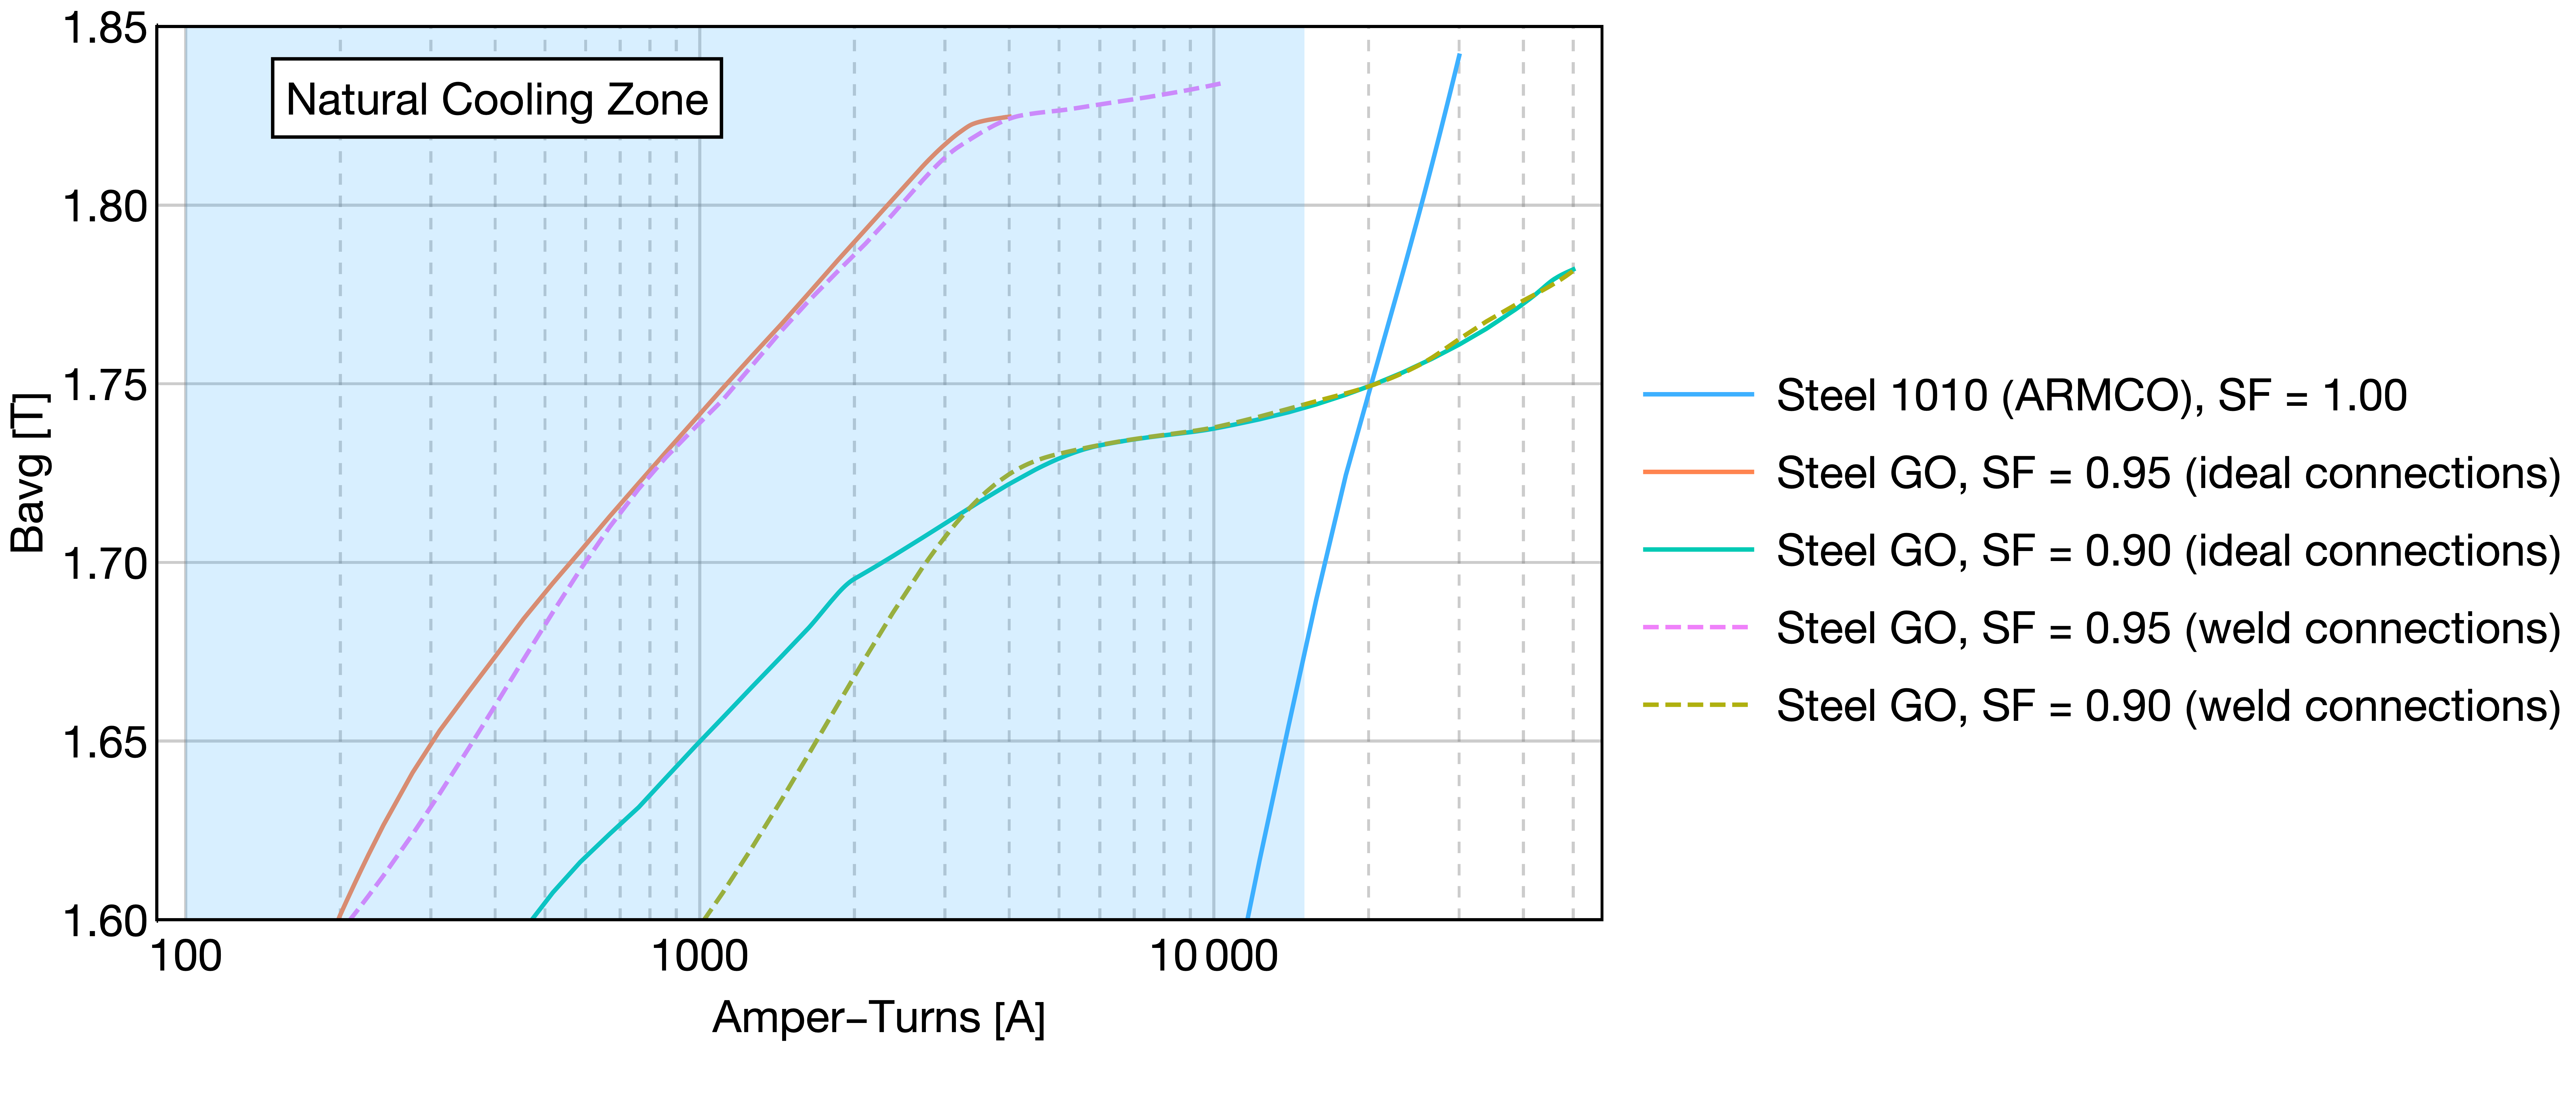
\includegraphics[width=0.8\columnwidth]{figs/Plot_2_logEx.png}
\caption{Magnetic field in the critical magnet region, as calculated for the magnet 1 of the shield, for different steel properties,
joint properties and stacking factors as a function of the total current in magnet coils. }
\label{fig:shieldEffectiveField}
\end{figure}

\begin{figure}[thbp]
\centering
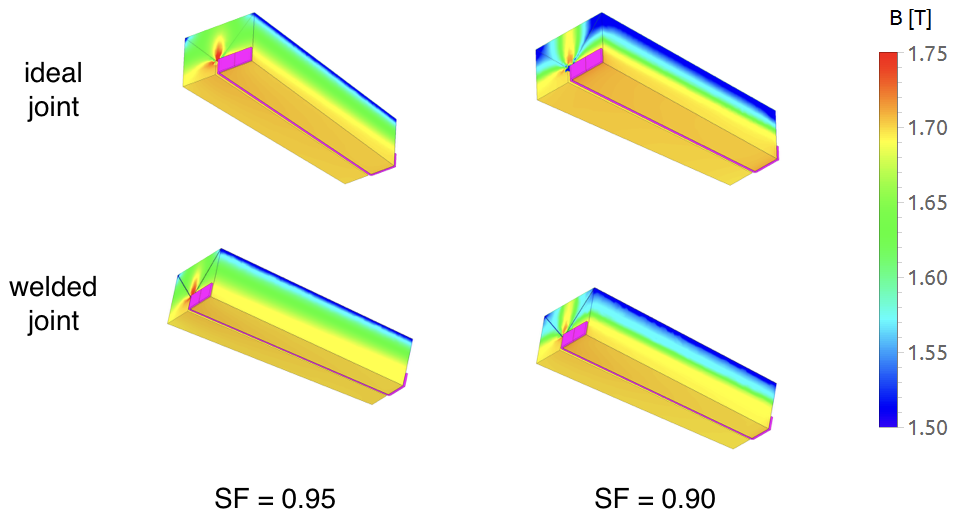
\includegraphics[width=0.8\columnwidth]{figs/shieldFieldModelling.png}
\caption{Modelled magnetic field map for ideal and welded joints, for stacking actors 95\% and 90\%. The current is set to provide effective magnetic field of 1.7 T in the critical magnet area.}
\label{fig:shieldEffectiveField}
\end{figure}

\begin{figure}[thbp]
\centering
%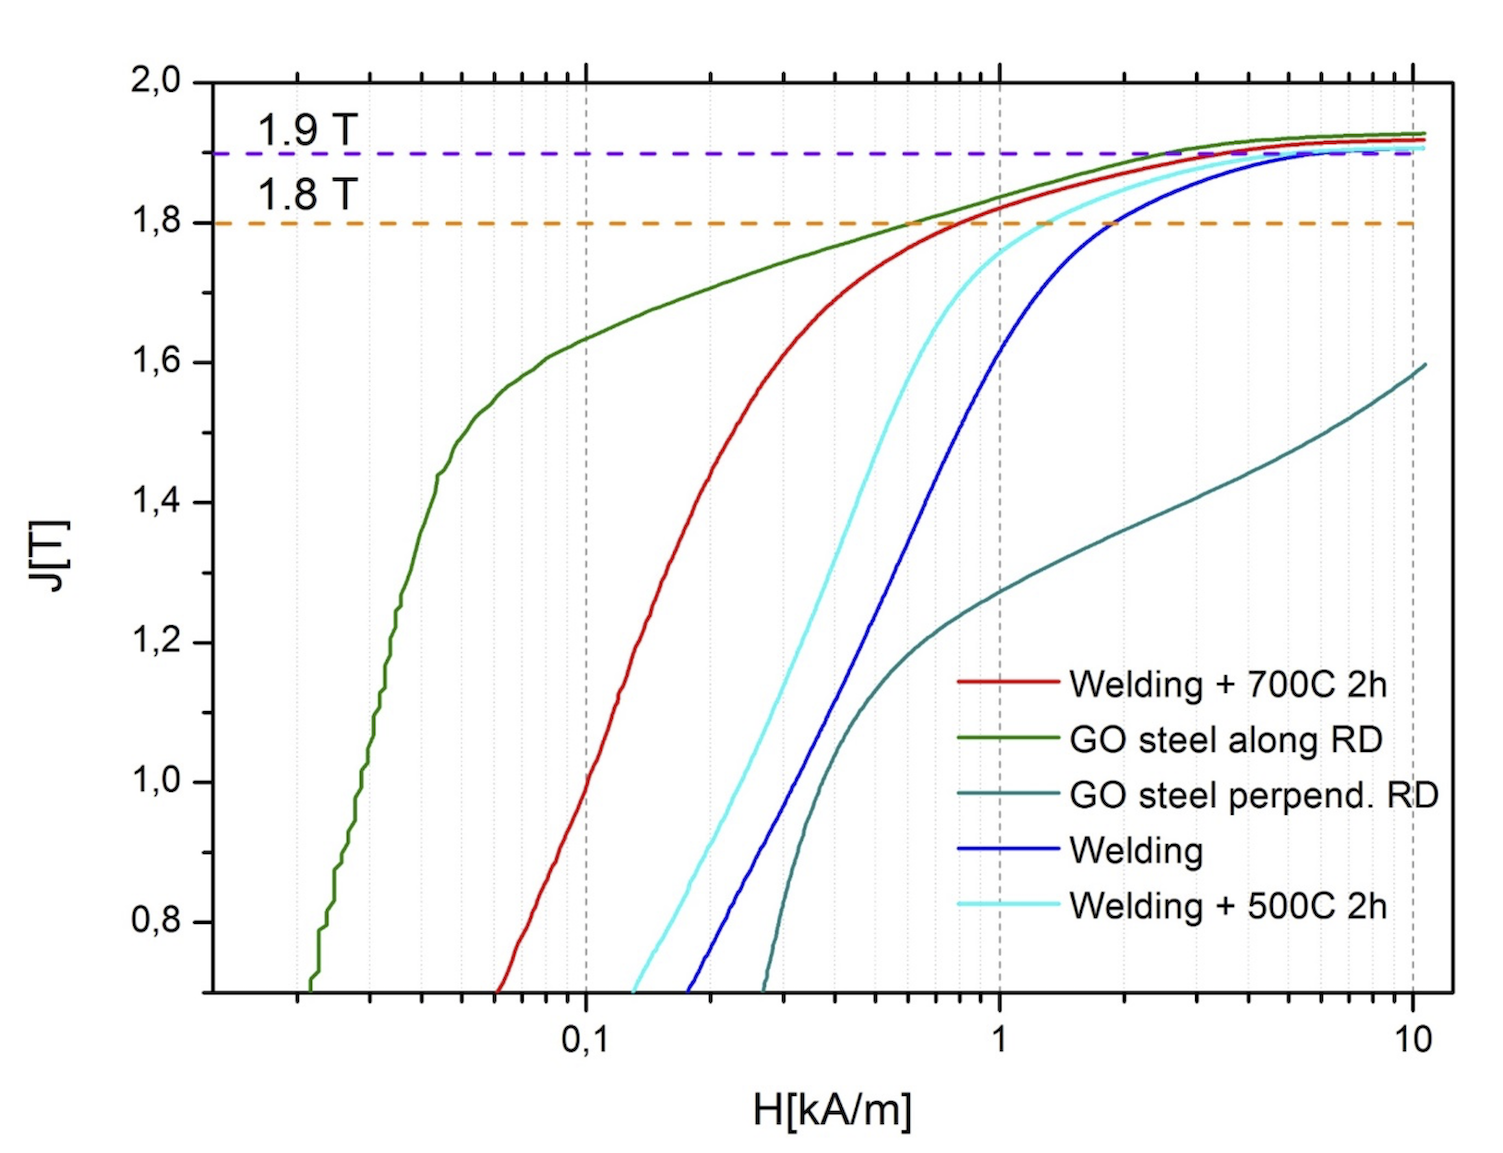
\includegraphics[width=1.0\columnwidth]{figs/go_steel_annealing.png}
\caption{Simulated hit rates caused by muons passing magnetic shield. Comparison of  ideal magnetic field setup (red) and realistic magnetic field (blue).}
\label{fig:shieldHitsMap}
\end{figure}

\begin{figure}[thbp] 
\centering
%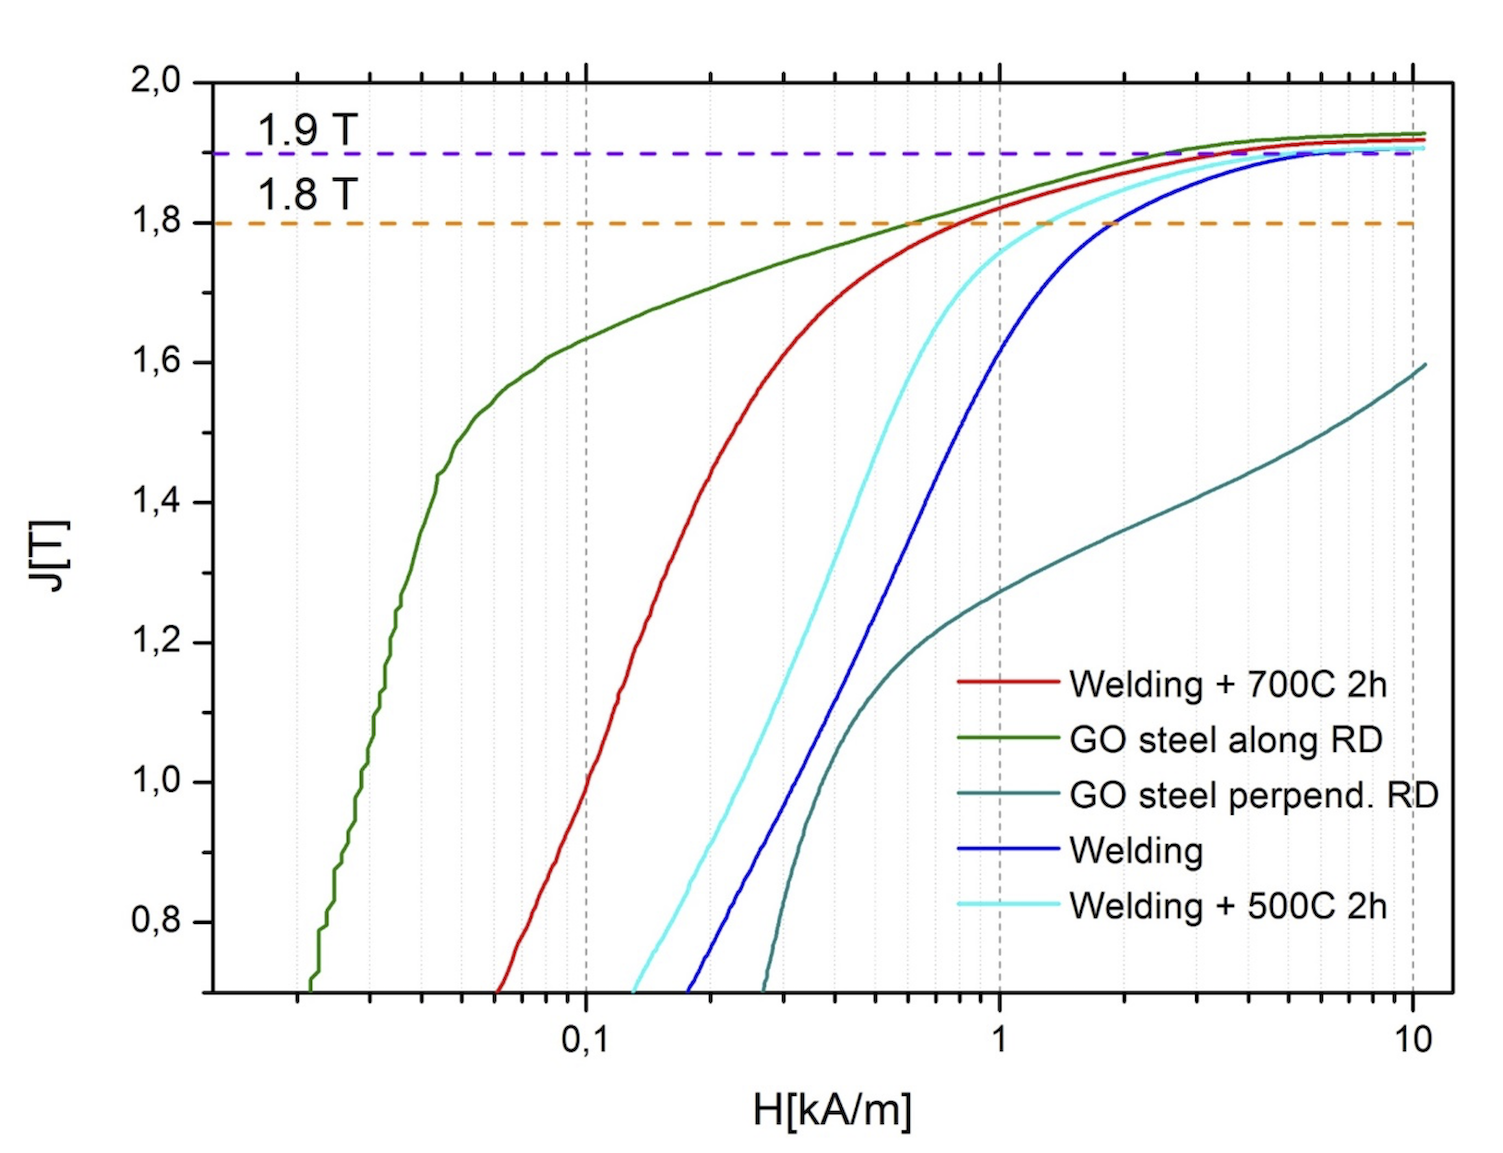
\includegraphics[width=1.0\columnwidth]{figs/go_steel_annealing.png}
\caption{Reconstructed track rates caused by muons passing magnetic shield. Comparison of  ideal magnetic field setup (red) and realistic magnetic field (blue).}
\label{fig:shieldTracks}
\end{figure}





\bibliographystyle{plain}
\bibliography{references}
\end{document}
